\documentclass[hyperref={bookmarks=false},aspectratio=169]{beamer}
\usepackage[utf8]{inputenc}

% ---------------  Define theme and color scheme  -----------------
\usetheme[sidebarleft]{Caltech}  % 3 options: minimal, sidebarleft, sidebarright

%\setbeamertemplate{footline}[frame number]

% ------------  Information on the title page  --------------------
\title[Grafička sučelja za git]
{\bfseries{Grafička sučelja za git}}



\author[Sandro Šafar \and Stella Dumenić\and Robin Šćulac]
{}

\institute[Riteh]


\date[25.1.2019.]
{Računalne vještine, računarstvo, 1. godina}
%------------------------------------------------------------

%------------------------------------------------------------
%The next block of commands puts the table of contents at the 
%beginning of each section and highlights the current section:

\AtBeginSection[]
{
  \begin{frame}
    \frametitle{Table of Contents}
    \tableofcontents[currentsection]
  \end{frame}
}
%------------------------------------------------------------


\begin{document}
\frame{\titlepage}  % Creates title page

%---------   table of contents after title page  ------------
%\begin{frame}
%\frametitle{Table of Contents}
%\tableofcontents
%\end{frame}
%---------------------------------------------------------


\section{gitflow}

\begin{frame}

\frametitle{Gitflow}
Gitflow je model grananja gita u kojem postoje dvije grane:

\begin{itemize}
    \item master 
    \item develop
\end{itemize}

Master grana je spremna za objavljivanje projekta dok develop grana služi za poboljšavanje ili dodavanje elemenata.

\end{frame}



\section{vrste gitflow sučelja}

%-----------------------------------------

%\begin{frame}
%\frametitle{TortoiseGit}


%\begin{itemize}
%    \item<1-> natuknice 
%    \item<2-> natuknice
%\end{itemize}

%\end{frame}

%-----------------------------------------------------
\begin{frame}
\frametitle{TortoiseGit}

\begin{block}{\tiny{Općenito}}
Open source sučelje namijenjeno za Windows
\end{block}
\begin{block}{Prednosti}

    \begin{itemize}
    \item jednostavan za koristiti 
    \item issue tracking system
    \item korisni alati
    \item dostupan u mnogo jezika
    \item stabilan
    \item sadrži spell check, auto completion
    \item besplatan za koristiti
    \end{itemize}
\end{block}
\end{frame}
%------------------------------------------------------

\begin{frame}
\frametitle{Aurees}

    
\begin{block}{\tiny{Općenito}}
Git sučelje namijenjeno za Windows i Mac korisnike. Uskoro dolazi verzija i za Linux.
\end{block}

\begin{block}{Prednosti}
    
    \begin{itemize}
        \item jednostavan za koristiti
        \item prikazuje commit-ove u "side by side" text editoru
        \item zanimljiv i jednostavan prikaz korisnika i izmjena
        \item besplatan za privatne korisnike
    \end{itemize}
\end{block}
\begin{figure}
    \centering
    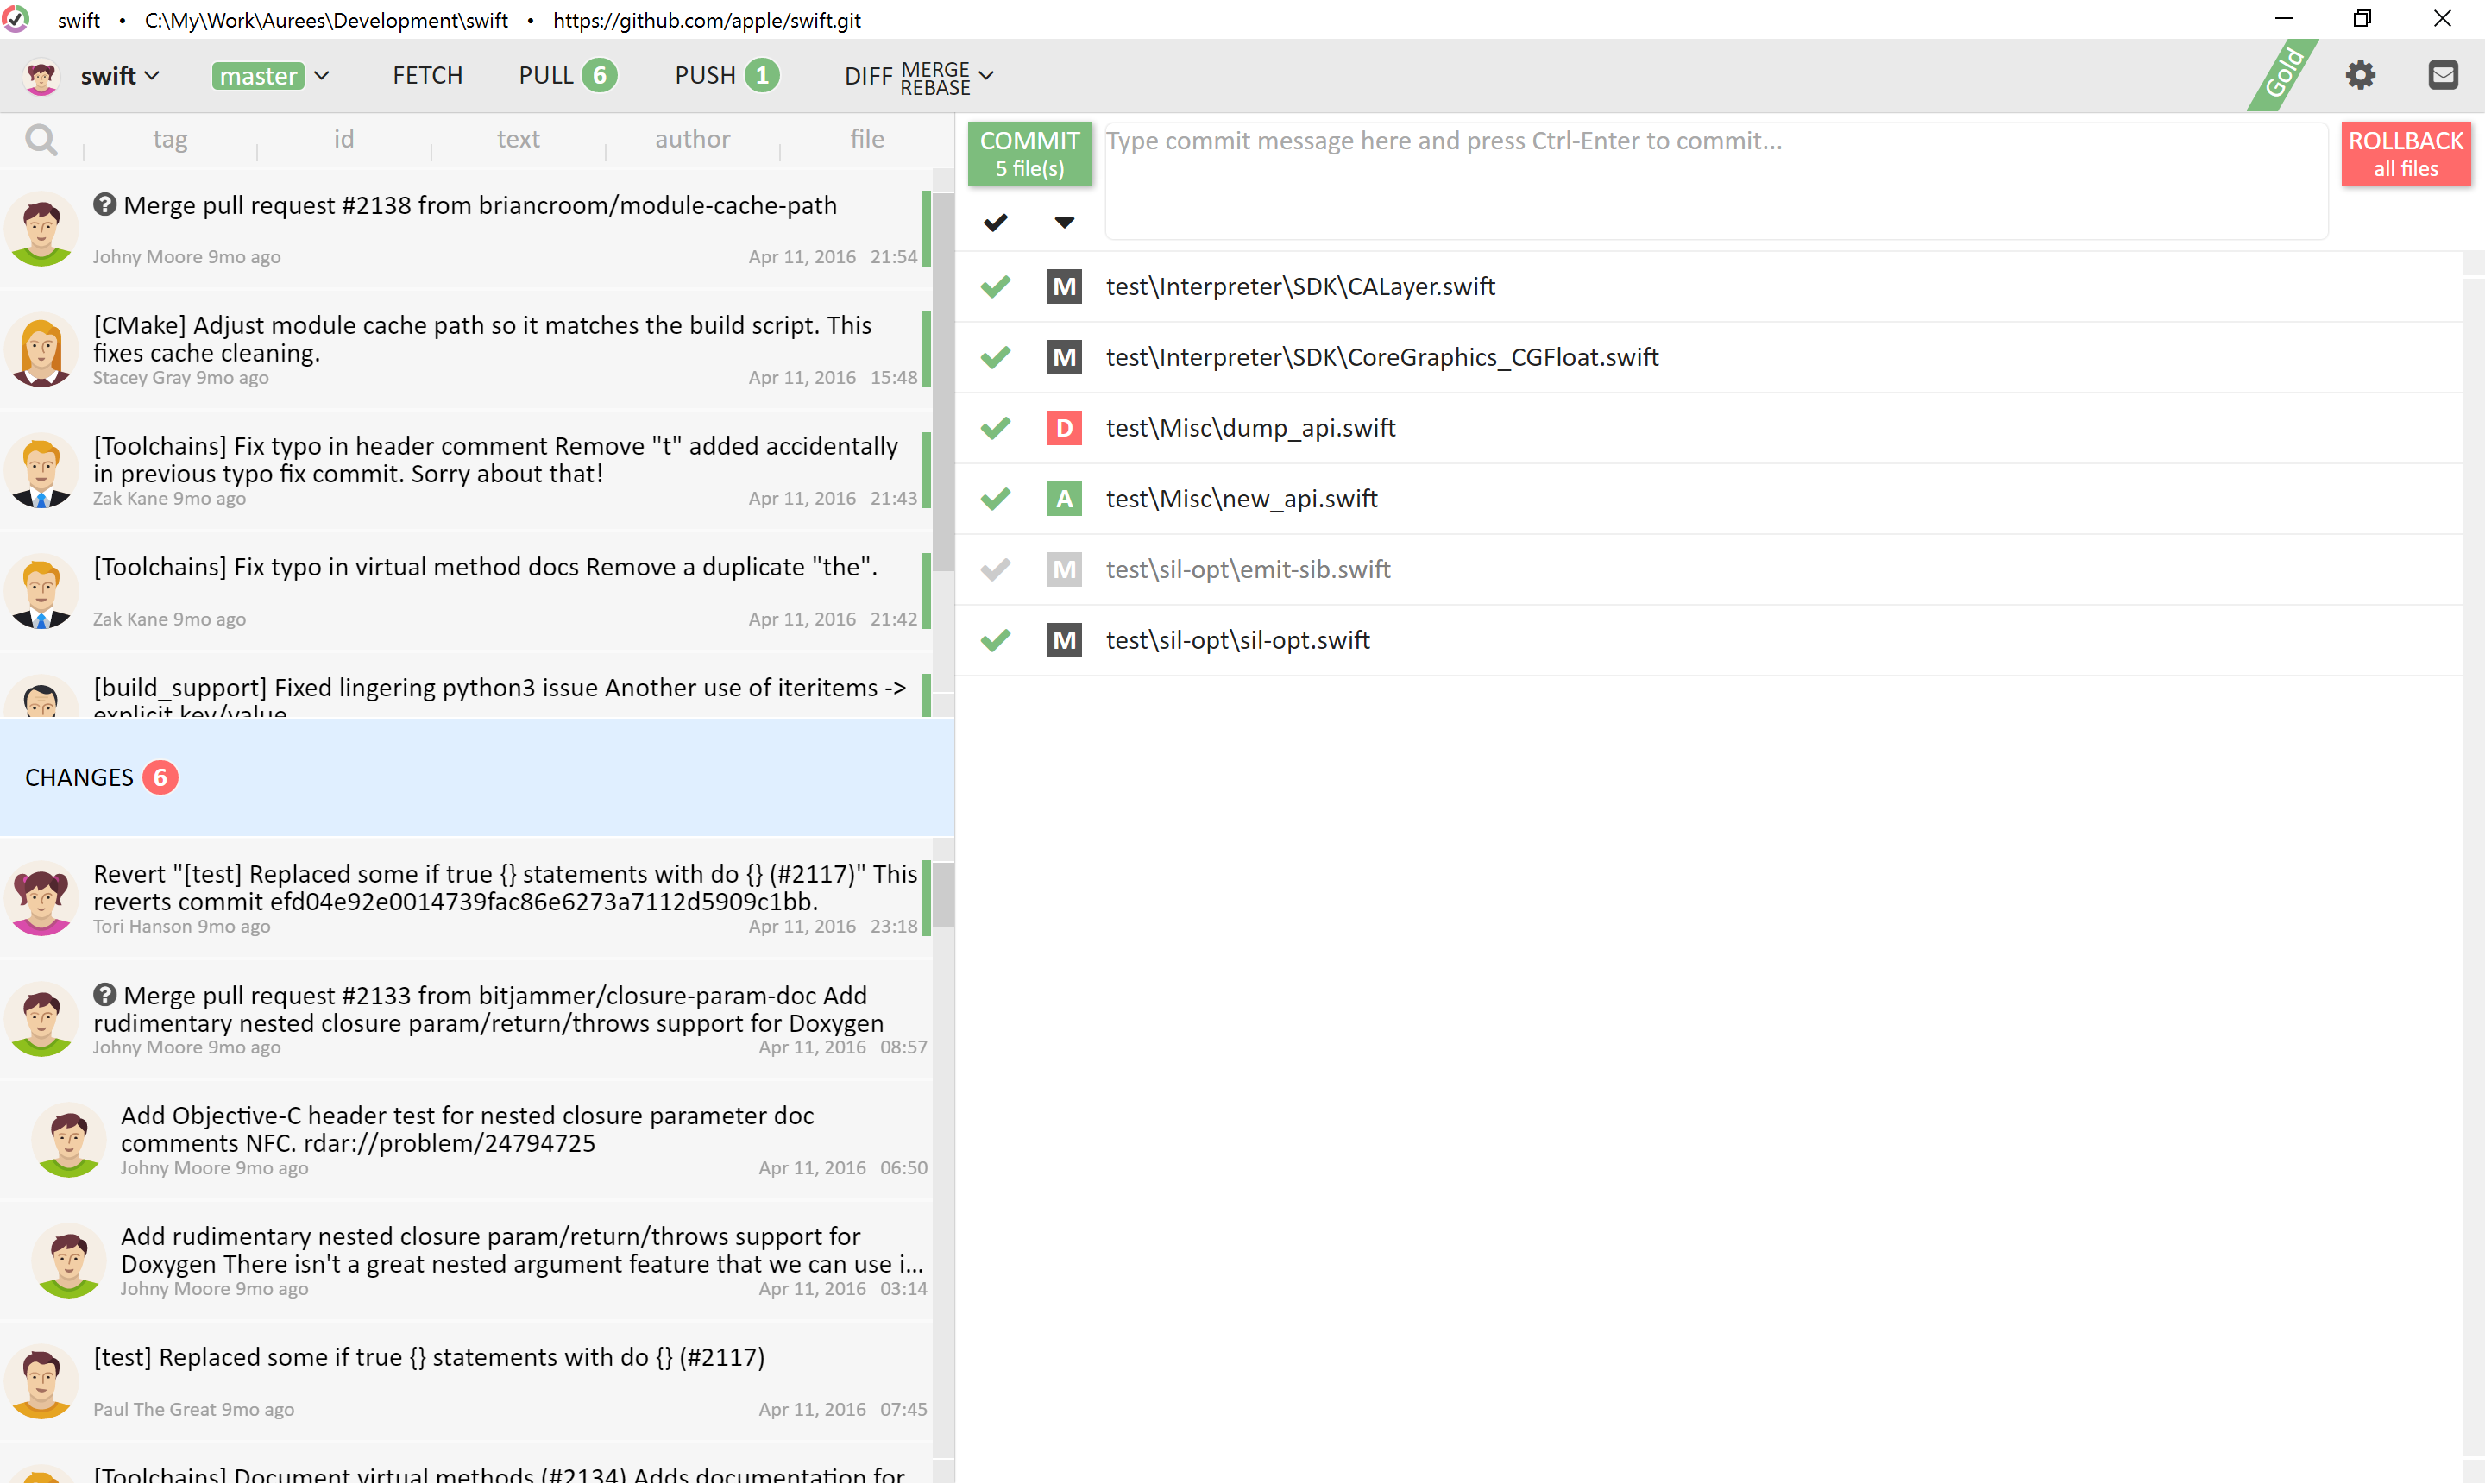
\includegraphics[width=100]{./figures/aurees.png}
    \caption{aurees}
\end{figure}
\end{frame}


%------------------------------------------------------kraken
\begin{frame}
\begin{columns}
\frametitle{GitKraken}
\column{0.45\textwidth}
\begin{figure}


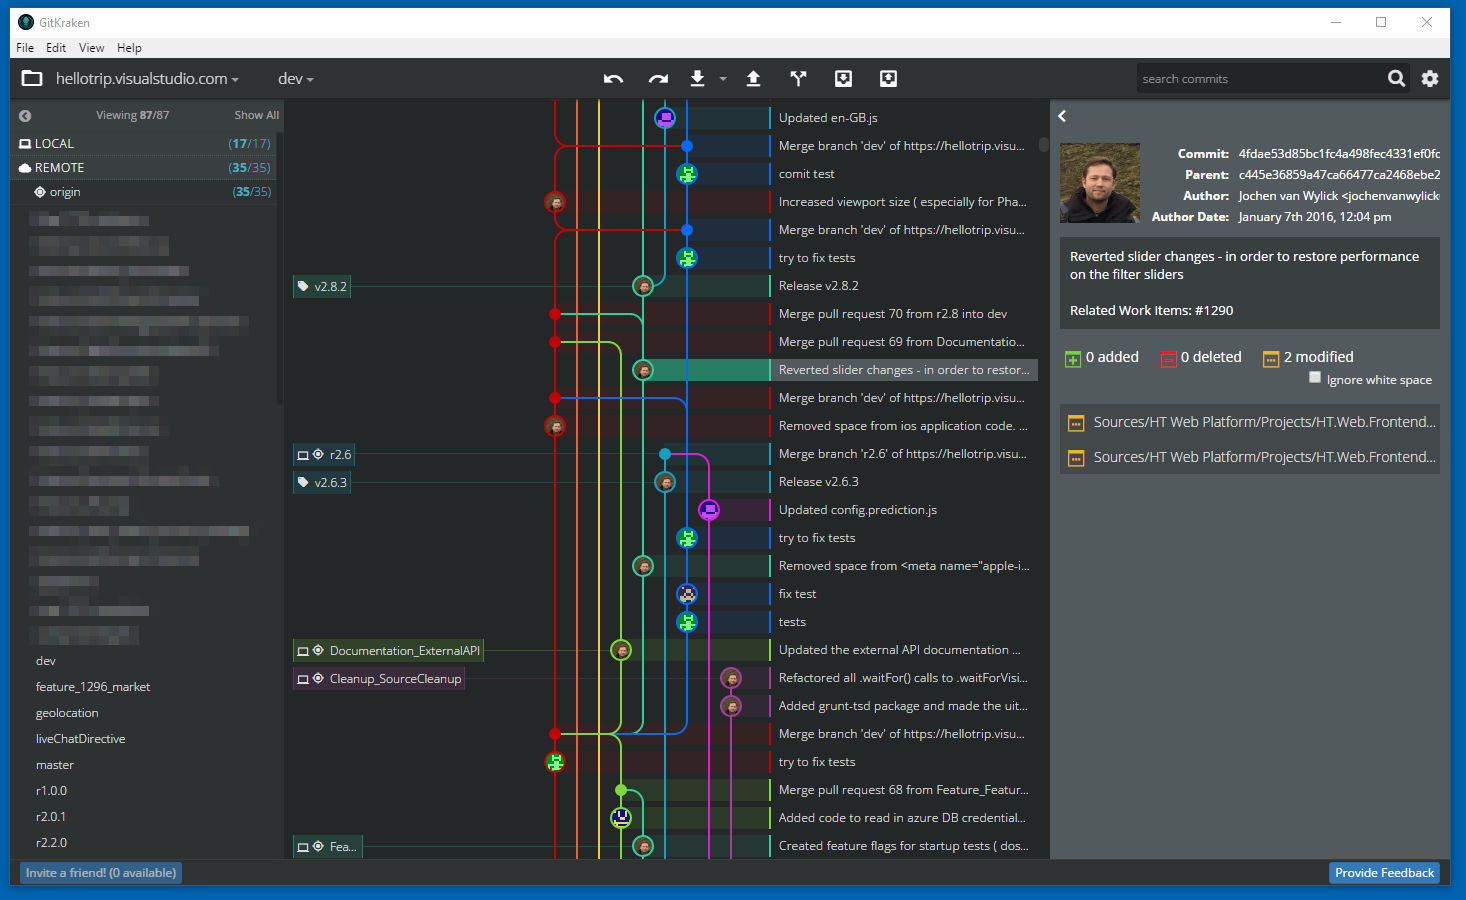
\includegraphics[width=\columnwidth]{./figures/git_kraken.png}
    \centering
    \caption{GUI od Git krakena  \emph{\\grafovi commit poruke i autori}}
\end{figure}
\column{0.55\textwidth}
GitKraken je git GUI sa korisničkoj intuitivnosti na umu sa svojim jednostavnim Drag & Drop sustavom olakšava puno naspram standardnog CLI-a. branchevi i povijest commitova je lako vidljiva uz GitKrakenov efikasan grafni prikaz.
\end{columns}

\end{frame}




%---------------------------------------------------------
\begin{frame}
\begin{columns}
\frametitle{GitHub Desktop}
\column{0.45\textwidth}
\begin{figure}


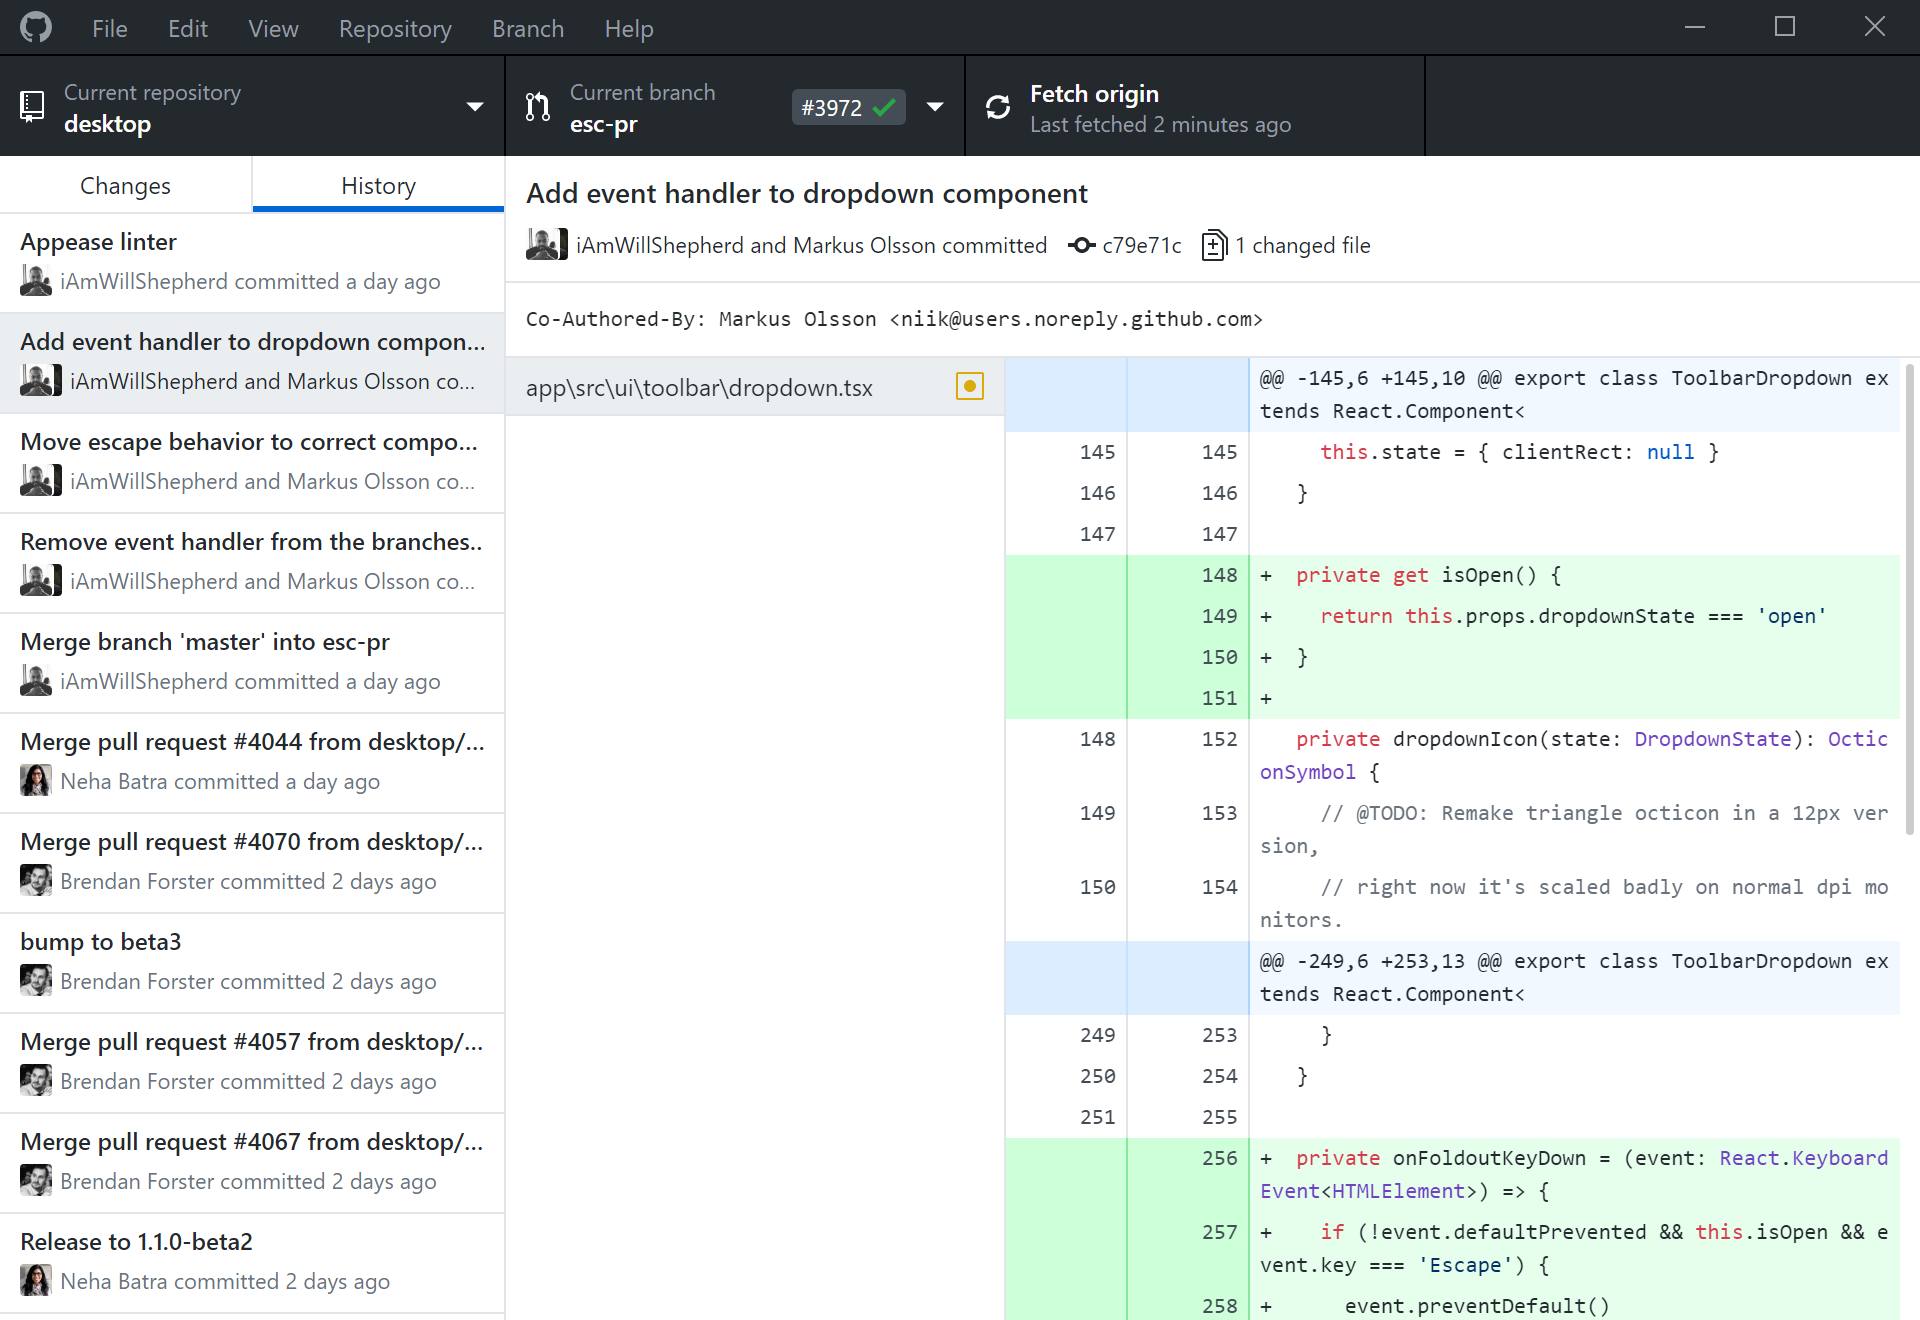
\includegraphics[width=\columnwidth]{./figures/github-desktop-screenshot-windows.png}
    \centering
    \caption{GUI od GitHubDesktopa  \emph{\\slika skinuta sa https://desktop.github.com/}}
\end{figure}
\column{0.55\textwidth}
\begin{itemize}
    \item ponaša se kao ekstenzija GitHuba i uz to olakšava pretraživanje GitHubovih repozitorija. Tokom commitova datoteke su pakirane nevjerovatnom brzinom (u uspordebi s GitKrakenom). 
    \item jedini nedostatci koje sam našao su da je nešto kompleksniji od ostalih GUI-a i ima ograničenje na slanju podataka
\end{itemize}
 
\end{columns}

\end{frame}

\end{document}
